% ============================================================
% 讲义 — 人教版七年级上册 第1章 有理数
% 编译命令：xelatex -interaction=nonstopmode 第1章_有理数.tex
% ============================================================
\documentclass[12pt, a4paper]{ctexart}
\usepackage[margin=2.2cm]{geometry}
\usepackage{amsmath, amssymb}
\usepackage{enumitem}
\usepackage{tcolorbox}
\usepackage{booktabs}
\usepackage{array}
\usepackage{fancyhdr}
\usepackage{xcolor}
\usepackage{tikz}
\usepackage{hyperref}
\usepackage{graphicx}
\usepackage{multirow}
\usepackage{pgfplots}
\pgfplotsset{compat=1.18}

% 颜色定义
\definecolor{mainblue}{RGB}{41, 98, 168}
\definecolor{lightblue}{RGB}{230, 240, 255}
\definecolor{tipgreen}{RGB}{34, 139, 87}
\definecolor{lightgreen}{RGB}{235, 250, 240}
\definecolor{warnred}{RGB}{200, 50, 50}
\definecolor{lightred}{RGB}{255, 240, 240}
\definecolor{examorange}{RGB}{210, 120, 20}
\definecolor{lightorange}{RGB}{255, 248, 235}
\definecolor{apppurple}{RGB}{120, 60, 170}
\definecolor{lightpurple}{RGB}{245, 238, 255}

% 页眉页脚
\pagestyle{fancy}
\fancyhf{}
\fancyhead[L]{\small\textcolor{mainblue}{\textbf{人教版七年级上册 · 第1章\quad 有理数}}}
\fancyhead[R]{\small\textcolor{mainblue}{家教讲义}}
\fancyfoot[C]{\small —\ \thepage\ —}
\renewcommand{\headrulewidth}{0.6pt}
\renewcommand{\headrule}{\hbox to\headwidth{\color{mainblue}\leaders\hrule height \headrulewidth\hfill}}
\renewcommand{\footrulewidth}{0pt}

% tcolorbox 样式
\newtcolorbox{knowledgebox}[1][]{%
  colback=lightblue, colframe=mainblue,
  fonttitle=\bfseries\large, title=#1,
  arc=3mm, boxrule=0.8pt,
  left=8pt, right=8pt, top=6pt, bottom=6pt
}

\newtcolorbox{tipbox}[1][]{%
  colback=lightgreen, colframe=tipgreen,
  fonttitle=\bfseries, title=#1,
  arc=2mm, boxrule=0.6pt,
  left=6pt, right=6pt, top=4pt, bottom=4pt
}

\newtcolorbox{warnbox}[1][]{%
  colback=lightred, colframe=warnred,
  fonttitle=\bfseries, title=#1,
  arc=2mm, boxrule=0.6pt,
  left=6pt, right=6pt, top=4pt, bottom=4pt
}

\newtcolorbox{examplebox}[1][]{%
  colback=lightorange, colframe=examorange,
  fonttitle=\bfseries, title=#1,
  arc=3mm, boxrule=0.8pt,
  left=8pt, right=8pt, top=6pt, bottom=6pt
}

\newtcolorbox{appbox}[1][]{%
  colback=lightpurple, colframe=apppurple,
  fonttitle=\bfseries, title=#1,
  arc=3mm, boxrule=0.8pt,
  left=8pt, right=8pt, top=6pt, bottom=6pt
}

\setCJKmainfont{Hiragino Sans GB}
\setCJKsansfont{Heiti SC}

\begin{document}

% ============ 标题页 ============
\begin{center}
{\Huge\bfseries\textcolor{mainblue}{第1章\quad 有理数}}\\[12pt]
{\Large\textcolor{gray}{家\quad 教\quad 讲\quad 义}}\\[8pt]
\rule{0.6\textwidth}{1pt}\\[8pt]
{\normalsize 适用：人教版\quad 七年级上册\quad |\quad 课时：4课时}
\end{center}
\vspace{10pt}

% ============================================================
%  第一部分：知识点讲解
% ============================================================
\section*{\textcolor{mainblue}{一、知识点讲解}}

\subsection*{1.1\quad 正数和负数}

\begin{knowledgebox}[正数和负数的概念]
\textbf{正数}：大于 $0$ 的数叫做正数，例如 $1,\ 2.5,\ \dfrac{3}{4},\ +100$ 等。正数前面的"$+$"号可以省略不写。

\textbf{负数}：在正数前面加上"$-$"号的数叫做负数，例如 $-1,\ -2.5,\ -\dfrac{3}{4},\ -100$ 等。负数前面的"$-$"号不能省略。

\textbf{零}：$0$ 既不是正数，也不是负数。$0$ 是正数和负数的分界点。
\end{knowledgebox}

\begin{warnbox}[易错提醒]
\begin{itemize}[leftmargin=*]
  \item $0$ 既不是正数也不是负数，不要把 $0$ 归为正数或负数！
  \item 带"$+$"号的不一定是正数，带"$-$"号的不一定是负数。例如 $-(-3) = 3$ 是正数，$-(+5) = -5$ 是负数。
  \item "$+$"和"$-$"有两种含义：一是表示\textbf{运算符号}（加、减），二是表示\textbf{性质符号}（正、负）。在 $(-3)+(+5)$ 中，第一个括号里的$-$是性质符号，中间的$+$是运算符号。
\end{itemize}
\end{warnbox}

\begin{knowledgebox}[用正负数表示相反意义的量]
在实际问题中，常用正数和负数来表示一对\textbf{具有相反意义的量}。例如：
\begin{itemize}[leftmargin=*]
  \item 温度：零上 $5\,^\circ\mathrm{C}$ 记作 $+5\,^\circ\mathrm{C}$，零下 $3\,^\circ\mathrm{C}$ 记作 $-3\,^\circ\mathrm{C}$
  \item 海拔：高于海平面 $100\,\mathrm{m}$ 记作 $+100\,\mathrm{m}$，低于海平面 $50\,\mathrm{m}$ 记作 $-50\,\mathrm{m}$
  \item 收支：收入 $200$ 元记作 $+200$ 元，支出 $80$ 元记作 $-80$ 元
  \item 方向：向东走 $3\,\mathrm{km}$ 记作 $+3\,\mathrm{km}$，向西走 $2\,\mathrm{km}$ 记作 $-2\,\mathrm{km}$
\end{itemize}
\end{knowledgebox}

\subsection*{1.2\quad 有理数的分类}

\begin{knowledgebox}[有理数的定义与分类]
\textbf{有理数}：整数和分数统称为有理数。

有理数可以按\textbf{定义}分类：
\begin{center}
\begin{tabular}{r|l}
\textbf{整数} & 正整数、$0$、负整数\\
\textbf{分数} & 正分数、负分数
\end{tabular}
\end{center}

有理数也可以按\textbf{符号}分类：
\begin{center}
\begin{tabular}{r|l}
\textbf{正有理数} & 正整数、正分数\\
\textbf{零} & $0$\\
\textbf{负有理数} & 负整数、负分数
\end{tabular}
\end{center}
\end{knowledgebox}

\begin{warnbox}[易错提醒]
\begin{itemize}[leftmargin=*]
  \item 有限小数和无限循环小数都是分数，因此都是有理数。例如 $0.333\cdots = \dfrac{1}{3}$ 是有理数。
  \item $\pi$ 不是有理数（它是无限不循环小数），但七年级阶段主要研究有理数。
  \item $-a$ 不一定是负数！当 $a$ 为负数时，$-a$ 是正数；当 $a = 0$ 时，$-a = 0$。
\end{itemize}
\end{warnbox}

\subsection*{1.3\quad 数轴}

\begin{knowledgebox}[数轴的定义与三要素]
\textbf{数轴}：规定了\textbf{原点}、\textbf{正方向}和\textbf{单位长度}的直线叫做数轴。

数轴的\textbf{三要素}，缺一不可：
\begin{enumerate}[leftmargin=*]
  \item \textbf{原点}：数轴上表示 $0$ 的点，用"$0$"标注。
  \item \textbf{正方向}：通常规定向右为正方向，用箭头表示。
  \item \textbf{单位长度}：数轴上相邻两个整数之间的距离，需保持一致。
\end{enumerate}

\begin{center}
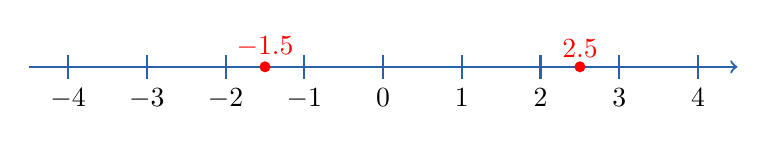
\begin{tikzpicture}
  \draw[->, thick, mainblue] (-4.5,0) -- (4.5,0);
  \foreach \x in {-4,-3,-2,-1,0,1,2,3,4}
    \draw[thick, mainblue] (\x, 0.15) -- (\x, -0.15);
  \node[below] at (0, -0.15) {$0$};
  \node[below] at (1, -0.15) {$1$};
  \node[below] at (2, -0.15) {$2$};
  \node[below] at (3, -0.15) {$3$};
  \node[below] at (4, -0.15) {$4$};
  \node[below] at (-1, -0.15) {$-1$};
  \node[below] at (-2, -0.15) {$-2$};
  \node[below] at (-3, -0.15) {$-3$};
  \node[below] at (-4, -0.15) {$-4$};
  \fill[red] (2.5,0) circle (2pt) node[above] {$2.5$};
  \fill[red] (-1.5,0) circle (2pt) node[above] {$-1.5$};
\end{tikzpicture}
\end{center}
\end{knowledgebox}

\begin{tipbox}[数轴上的大小关系]
数轴上右边的数总比左边的数大。即若点 $A$ 在点 $B$ 的右边，则 $A > B$。

\textbf{结论}：正数 $> 0 >$ 负数；两个负数，绝对值大的反而小。
\end{tipbox}

\subsection*{1.4\quad 相反数}

\begin{knowledgebox}[相反数的定义]
\textbf{相反数}：只有符号不同的两个数互为相反数。$a$ 的相反数是 $-a$。

\begin{itemize}[leftmargin=*]
  \item 互为相反数的两个数之和为 $0$，即 $a + (-a) = 0$。
  \item $0$ 的相反数是 $0$。
  \item 互为相反数的两个数的绝对值相等，即 $|a| = |-a|$。
\end{itemize}

在数轴上，互为相反数的两个数位于原点的两侧，且到原点的距离相等。
\end{knowledgebox}

\subsection*{1.5\quad 绝对值}

\begin{knowledgebox}[绝对值的定义]
\textbf{绝对值}：数轴上表示数 $a$ 的点与原点的\textbf{距离}叫做数 $a$ 的绝对值，记作 $|a|$。

\[
|a| = \begin{cases} a, & \text{当 } a > 0 \\ 0, & \text{当 } a = 0 \\ -a, & \text{当 } a < 0 \end{cases}
\]

\textbf{性质}：
\begin{enumerate}[leftmargin=*]
  \item 绝对值具有\textbf{非负性}：$|a| \geqslant 0$，即任何数的绝对值都是非负数。
  \item 互为相反数的绝对值相等：$|a| = |-a|$。
  \item 若 $|a| = a$，则 $a \geqslant 0$；若 $|a| = -a$，则 $a \leqslant 0$。
\end{enumerate}
\end{knowledgebox}

\begin{warnbox}[易错提醒]
\begin{itemize}[leftmargin=*]
  \item $|a|$ 一定是非负数，不可能为负数。
  \item $-|a|$ 一定是非正数（$\leqslant 0$）。
  \item $|a - b|$ 表示数轴上 $a$、$b$ 两点之间的距离。
  \item 若 $|a| = 3$，则 $a = 3$ 或 $a = -3$（注意两个解）。
\end{itemize}
\end{warnbox}

\subsection*{1.6\quad 有理数的加减法}

\begin{knowledgebox}[有理数加法法则]
\begin{enumerate}[leftmargin=*]
  \item \textbf{同号两数相加}：取相同的符号，并把绝对值相加。\\
  例：$(-3) + (-5) = -8$，$(+3) + (+5) = +8$
  \item \textbf{异号两数相加}：取绝对值较大的加数的符号，并用较大的绝对值减去较小的绝对值。\\
  例：$(-7) + (+3) = -4$，$(+7) + (-3) = +4$
  \item \textbf{一个数与 $0$ 相加}：仍得这个数。\\
  例：$(-5) + 0 = -5$，$0 + 0 = 0$
  \item \textbf{互为相反数的两数相加得 $0$}。\\
  例：$(-3) + (+3) = 0$
\end{enumerate}
\end{knowledgebox}

\begin{knowledgebox}[有理数减法法则]
减去一个数等于加上这个数的\textbf{相反数}：
\[
a - b = a + (-b)
\]
例：$(-3) - (-5) = (-3) + (+5) = 2$
\end{knowledgebox}

\begin{tipbox}[加减法的运算技巧]
\begin{itemize}[leftmargin=*]
  \item 减法统一转化为加法，再用加法法则计算。
  \item 遇到多个有理数相加减，可以将正数和负数分别相加，再把结果相加（"归类法"）。
  \item 有相反数的先配对，可以简化计算。
\end{itemize}
\end{tipbox}

\subsection*{1.7\quad 有理数的乘除法}

\begin{knowledgebox}[有理数乘法法则]
\begin{enumerate}[leftmargin=*]
  \item \textbf{同号得正}：两数相乘，同号取正号，并把绝对值相乘。\\
  $(-3) \times (-4) = +12$，$(+3) \times (+4) = +12$
  \item \textbf{异号得负}：两数相乘，异号取负号，并把绝对值相乘。\\
  $(-3) \times (+4) = -12$，$(+3) \times (-4) = -12$
  \item 任何数与 $0$ 相乘，积为 $0$。\\
  $a \times 0 = 0$
\end{enumerate}
\end{knowledgebox}

\begin{knowledgebox}[有理数除法法则]
除以一个不为零的数等于乘以这个数的\textbf{倒数}：
\[
a \div b = a \times \frac{1}{b} \quad (b \neq 0)
\]
\textbf{符号法则与乘法相同}：同号得正，异号得负。
\end{knowledgebox}

\begin{tipbox}[倒数的概念]
乘积为 $1$ 的两个数互为\textbf{倒数}。$a$ 的倒数为 $\dfrac{1}{a}$（$a \neq 0$）。

注意：$0$ 没有倒数；互为倒数的两个数同号。
\end{tipbox}

\begin{warnbox}[易错提醒]
\begin{itemize}[leftmargin=*]
  \item 多个有理数相乘时，先确定符号：负因数的个数为\textbf{偶数}个时积为正，为\textbf{奇数}个时积为负。
  \item $0$ 没有倒数，除数不能为 $0$。
  \item $a \div (b + c) \neq a \div b + a \div c$，除法没有分配律！
\end{itemize}
\end{warnbox}

\subsection*{1.8\quad 有理数的乘方}

\begin{knowledgebox}[乘方的定义]
$n$ 个相同的因数 $a$ 相乘，记作 $a^n$，读作"$a$ 的 $n$ 次方"或"$a$ 的 $n$ 次幂"：
\[
\underbrace{a \times a \times \cdots \times a}_{n\text{个}} = a^n
\]
其中 $a$ 叫做\textbf{底数}，$n$ 叫做\textbf{指数}，$a^n$ 叫做\textbf{幂}。

\textbf{特别规定}：
\begin{itemize}[leftmargin=*]
  \item $a^1 = a$（任何数的 $1$ 次方等于它本身）
  \item $a^0 = 1$（任何非零数的 $0$ 次方等于 $1$；七年级可暂不深入）
\end{itemize}
\end{knowledgebox}

\begin{warnbox}[易错提醒]
\begin{itemize}[leftmargin=*]
  \item $(-2)^2 = (-2) \times (-2) = 4$，而 $-2^2 = -(2 \times 2) = -4$。括号的位置很重要！
  \item $(-1)^n$：$n$ 为偶数时结果为 $1$，$n$ 为奇数时结果为 $-1$。
  \item 负数的偶次幂为正，奇次幂为负。
\end{itemize}
\end{warnbox}

\subsection*{1.9\quad 有理数的混合运算顺序}

\begin{knowledgebox}[混合运算顺序]
有理数的混合运算，按以下顺序进行：
\begin{enumerate}[leftmargin=*]
  \item 先算\textbf{乘方}（三级运算）
  \item 再算\textbf{乘除}（二级运算）
  \item 最后算\textbf{加减}（一级运算）
  \item 有括号的，先算\textbf{小括号}，再算\textbf{中括号}，最后算\textbf{大括号}
  \item 同级运算，从\textbf{左到右}依次计算
\end{enumerate}

口诀：\textbf{先乘方，后乘除，再加减；有括号，先括号。}
\end{knowledgebox}

\subsection*{1.10\quad 科学记数法}

\begin{knowledgebox}[科学记数法]
把一个大于 $10$ 的数记成 $a \times 10^n$ 的形式（其中 $1 \leqslant |a| < 10$，$n$ 为正整数），这种记数方法叫做\textbf{科学记数法}。

\textbf{确定 $n$ 的方法}：$n$ 等于原数的整数部分位数减 $1$。

\textbf{举例}：
\begin{itemize}[leftmargin=*]
  \item $300\,000 = 3 \times 10^5$（$6$ 位数，$n = 6 - 1 = 5$）
  \item $4\,500\,000 = 4.5 \times 10^6$（$7$ 位数，$n = 7 - 1 = 6$）
  \item $7\,280\,000\,000 = 7.28 \times 10^9$（$10$ 位数，$n = 10 - 1 = 9$）
\end{itemize}
\end{knowledgebox}

\begin{tipbox}[科学记数法小技巧]
\begin{itemize}[leftmargin=*]
  \item 较小的正数（$0 < x < 1$）也可以用科学记数法表示，此时 $n$ 为负整数。\\
  例：$0.00035 = 3.5 \times 10^{-4}$
  \item 科学记数法还原时，$10^n$ 表示小数点向右移动 $n$ 位。
\end{itemize}
\end{tipbox}


% ============================================================
%  第二部分：例题精讲
% ============================================================
\section*{\textcolor{examorange}{二、例题精讲}}

\begin{examplebox}[【例题1】有理数的加减混合计算]
计算：$(-3) + (+7) - (-2) + (-5) - (+1)$
\end{examplebox}

\textbf{解}：先将减法统一转化为加法：
\[
(-3) + (+7) - (-2) + (-5) - (+1) = (-3) + (+7) + (+2) + (-5) + (-1)
\]
将正数和负数分别归类：
\[
= [(+7) + (+2)] + [(-3) + (-5) + (-1)] = (+9) + (-9) = 0
\]

\begin{tipbox}[方法总结]
加减混合运算的关键步骤：(1) 减法转化为加法；(2) 正数、负数分别归类求和；(3) 最后将两组结果相加。
\end{tipbox}

\vspace{6pt}

\begin{examplebox}[【例题2】有理数乘除法与符号判断]
计算：$(-2) \times (-3) \times (-4) \div (-6)$
\end{examplebox}

\textbf{解}：先确定符号。负因数有 $3$ 个（奇数个），因此结果为\textbf{负}。

绝对值：$2 \times 3 \times 4 \div 6 = 24 \div 6 = 4$

所以原式 $= -4$。

\begin{tipbox}[方法总结]
多个有理数相乘除时，先数负因数个数定符号（偶正奇负），再计算绝对值。乘除法属于同级运算，从左到右依次计算。
\end{tipbox}

\vspace{6pt}

\begin{examplebox}[【例题3】乘方运算与符号辨析]
计算下列各式：
\begin{enumerate}[leftmargin=*]
  \item $(-2)^4$
  \item $-2^4$
  \item $(-1)^{2025}$
  \item $\left(-\dfrac{2}{3}\right)^3$
\end{enumerate}
\end{examplebox}

\textbf{解}：
\begin{enumerate}[leftmargin=*]
  \item $(-2)^4 = (-2) \times (-2) \times (-2) \times (-2) = 16$（底数是 $-2$，指数 $4$ 是偶数，结果为正）
  \item $-2^4 = -(2 \times 2 \times 2 \times 2) = -16$（底数是 $2$，不是 $-2$！先算 $2^4$ 再取负）
  \item $(-1)^{2025} = -1$（$2025$ 是奇数）
  \item $\left(-\dfrac{2}{3}\right)^3 = -\dfrac{2^3}{3^3} = -\dfrac{8}{27}$（底数是 $-\dfrac{2}{3}$，指数 $3$ 是奇数，结果为负）
\end{enumerate}

\begin{tipbox}[方法总结]
区分 $(-a)^n$ 和 $-a^n$：前者底数包含负号，后者底数不含负号。$(-a)^n$ 的符号取决于 $n$ 的奇偶性。
\end{tipbox}

\vspace{6pt}

\begin{examplebox}[【例题4】绝对值的化简]
已知 $a < 0$，化简 $|a| + |a - 3|$。
\end{examplebox}

\textbf{解}：因为 $a < 0$，所以：
\begin{itemize}[leftmargin=*]
  \item $|a| = -a$（负数的绝对值是它的相反数）
  \item 因为 $a < 0$，所以 $a - 3 < 0$，故 $|a - 3| = -(a-3) = 3 - a$
\end{itemize}
因此：
\[
|a| + |a - 3| = (-a) + (3 - a) = 3 - 2a
\]

\begin{tipbox}[方法总结]
绝对值化简的关键是判断绝对值里面的式子是正还是负。正数取本身，负数取相反数。此题需要根据 $a < 0$ 的条件逐一判断。
\end{tipbox}

\vspace{6pt}

\begin{examplebox}[【例题5】技巧性计算——凑整与分配律]
用简便方法计算：$99 \times \left(-\dfrac{5}{7}\right) + \left(-\dfrac{5}{7}\right) \times (-5)$
\end{examplebox}

\textbf{解}：提取公因数 $\left(-\dfrac{5}{7}\right)$（逆用分配律）：
\[
99 \times \left(-\frac{5}{7}\right) + \left(-\frac{5}{7}\right) \times (-5)
= \left(-\frac{5}{7}\right) \times [99 + (-5)]
= \left(-\frac{5}{7}\right) \times 94
= -\frac{470}{7}
= -67\frac{1}{7}
\]

\begin{tipbox}[方法总结]
简便计算常用技巧：(1) \textbf{凑整法}——将接近整十整百的数拆开；(2) \textbf{逆用分配律}——提取公因数 $ab + ac = a(b+c)$；(3) \textbf{交换结合}——利用加法交换律和结合律，将容易计算的数先配对。
\end{tipbox}

\vspace{6pt}

\begin{examplebox}[【例题6】混合运算综合]
计算：$-2^2 + (-2)^3 \times \left(-\dfrac{1}{2}\right) - (-1)^{10}$
\end{examplebox}

\textbf{解}：按运算顺序，先算乘方：
\begin{align*}
-2^2 &= -4 \\
(-2)^3 &= -8 \\
(-1)^{10} &= 1
\end{align*}
代入原式：
\[
-4 + (-8) \times \left(-\frac{1}{2}\right) - 1 = -4 + 4 - 1 = -1
\]

\begin{tipbox}[方法总结]
混合运算务必严格遵守运算顺序：先乘方，再乘除，最后加减。特别注意 $-2^2 \neq (-2)^2$，以及 $(-1)$ 的偶次幂为 $1$。
\end{tipbox}

\vspace{6pt}

\begin{examplebox}[【例题7】数轴与绝对值的综合]
在数轴上，点 $A$ 表示 $-3$，点 $B$ 表示 $5$。求 $A$、$B$ 两点之间的距离。
\end{examplebox}

\textbf{解}：$A$、$B$ 两点之间的距离为：
\[
|5 - (-3)| = |5 + 3| = |8| = 8
\]

\begin{tipbox}[方法总结]
数轴上两点 $A(a)$、$B(b)$ 之间的距离公式：$AB = |a - b|$。这个公式无论 $a$、$b$ 谁大谁小都成立。
\end{tipbox}


% ============================================================
%  第三部分：应用题
% ============================================================
\section*{\textcolor{apppurple}{三、应用题}}

\begin{appbox}[【应用1】温度问题]
某天早晨的气温是 $-5\,^\circ\mathrm{C}$，到中午上升了 $12\,^\circ\mathrm{C}$，到傍晚又下降了 $7\,^\circ\mathrm{C}$。问：傍晚的气温是多少摄氏度？
\end{appbox}

\textbf{解}：
\[
-5 + 12 + (-7) = -5 + 12 - 7 = 0\,(^\circ\mathrm{C})
\]

答：傍晚的气温是 $0\,^\circ\mathrm{C}$。

\begin{appbox}[【应用2】财务收支问题]
小明的妈妈记录了家里一周的收支情况：周一收入 $200$ 元，周二支出 $150$ 元，周三支出 $80$ 元，周四收入 $300$ 元，周五支出 $120$ 元，周六收入 $50$ 元，周日支出 $200$ 元。
\begin{enumerate}[leftmargin=*]
  \item 如果把收入记为正、支出记为负，请用正负数表示每天的收支。
  \item 这一周合计是盈利还是亏损？金额是多少？
\end{enumerate}
\end{appbox}

\textbf{解}：
\begin{enumerate}[leftmargin=*]
  \item 周一 $+200$，周二 $-150$，周三 $-80$，周四 $+300$，周五 $-120$，周六 $+50$，周日 $-200$。
  \item 合计：$(+200) + (-150) + (-80) + (+300) + (-120) + (+50) + (-200)$\\
  $= (200 + 300 + 50) + [(-150) + (-80) + (-120) + (-200)]$\\
  $= 550 + (-550) = 0$（元）
\end{enumerate}

答：这一周收支平衡，既没有盈利也没有亏损。

\begin{appbox}[【应用3】海拔与深度问题]
一架飞机在海拔 $8000\,\mathrm{m}$ 的高空飞行，一艘潜艇在飞机正下方的海面以下 $200\,\mathrm{m}$ 处潜行。
\begin{enumerate}[leftmargin=*]
  \item 如果以海平面为基准，飞机和潜艇的高度分别记为多少？
  \item 飞机与潜艇之间的垂直距离是多少米？
\end{enumerate}
\end{appbox}

\textbf{解}：
\begin{enumerate}[leftmargin=*]
  \item 以海平面为基准（海平面高度为 $0$），飞机高度为 $+8000\,\mathrm{m}$，潜艇高度为 $-200\,\mathrm{m}$。
  \item 垂直距离：$|8000 - (-200)| = |8000 + 200| = 8200\,(\mathrm{m})$
\end{enumerate}

答：飞机与潜艇之间的垂直距离是 $8200\,\mathrm{m}$。

\begin{appbox}[【应用4】科学记数法的实际应用]
据新闻报道，2024年我国某城市的年接待游客量达到 $128\,000\,000$ 人次，全年旅游收入达到 $156\,400\,000\,000$ 元。请用科学记数法表示这两个数据。
\end{appbox}

\textbf{解}：
\begin{itemize}[leftmargin=*]
  \item $128\,000\,000 = 1.28 \times 10^8$（人次）
  \item $156\,400\,000\,000 = 1.564 \times 10^{11}$（元）
\end{itemize}


% ============================================================
%  第四部分：课堂练习与参考答案
% ============================================================
\section*{\textcolor{tipgreen}{四、课堂练习}}

\begin{enumerate}[leftmargin=*]
  \item 计算：$(-8) + (+3) - (-5) + (-2)$

  \item 计算：$(-3)^2 - (-2)^3 + (-1)^{100}$

  \item 已知 $|a| = 4$，$|b| = 2$，且 $a < 0$，$b > 0$，求 $a + b$ 和 $a \times b$ 的值。

  \item 用简便方法计算：$(-12.5) \times 8 \times (-4)$

  \item 某冷库的温度是 $-18\,^\circ\mathrm{C}$，一批食品需要降温到 $-25\,^\circ\mathrm{C}$ 才能保存。问：温度还需降低多少度？
\end{enumerate}

\vspace{10pt}

\begin{knowledgebox}[参考答案]
\textbf{第1题}：
\[
(-8) + (+3) - (-5) + (-2) = (-8) + 3 + 5 + (-2) = (-8) + (-2) + 3 + 5 = -10 + 8 = -2
\]

\textbf{第2题}：
\[
(-3)^2 - (-2)^3 + (-1)^{100} = 9 - (-8) + 1 = 9 + 8 + 1 = 18
\]

\textbf{第3题}：

因为 $|a|=4$ 且 $a<0$，所以 $a = -4$。因为 $|b|=2$ 且 $b>0$，所以 $b = 2$。

$a + b = -4 + 2 = -2$；$a \times b = (-4) \times 2 = -8$

\textbf{第4题}：
\[
(-12.5) \times 8 \times (-4) = [(-12.5) \times (-4)] \times 8 = 50 \times 8 = 400
\]
（利用乘法交换律，先算 $(-12.5) \times (-4) = 50$，凑整后再乘 $8$）

\textbf{第5题}：

需要降低的温度：$(-25) - (-18) = -25 + 18 = -7\,(^\circ\mathrm{C})$

答：温度还需降低 $7\,^\circ\mathrm{C}$。
\end{knowledgebox}

\vfill
\begin{center}
\small\textcolor{gray}{本讲义仅供教学参考，例题可根据学生水平调整难度。}
\end{center}

\end{document}
